% Modeling
\section{One Dimensional Wave Equation}

In this section the one dimensional wave equation for a linear elastic material with uniform density and cross-sectional area will be derived. The derivation is based on knowledge from a number of published sources.

\begin{figure}[ht!]
\centering
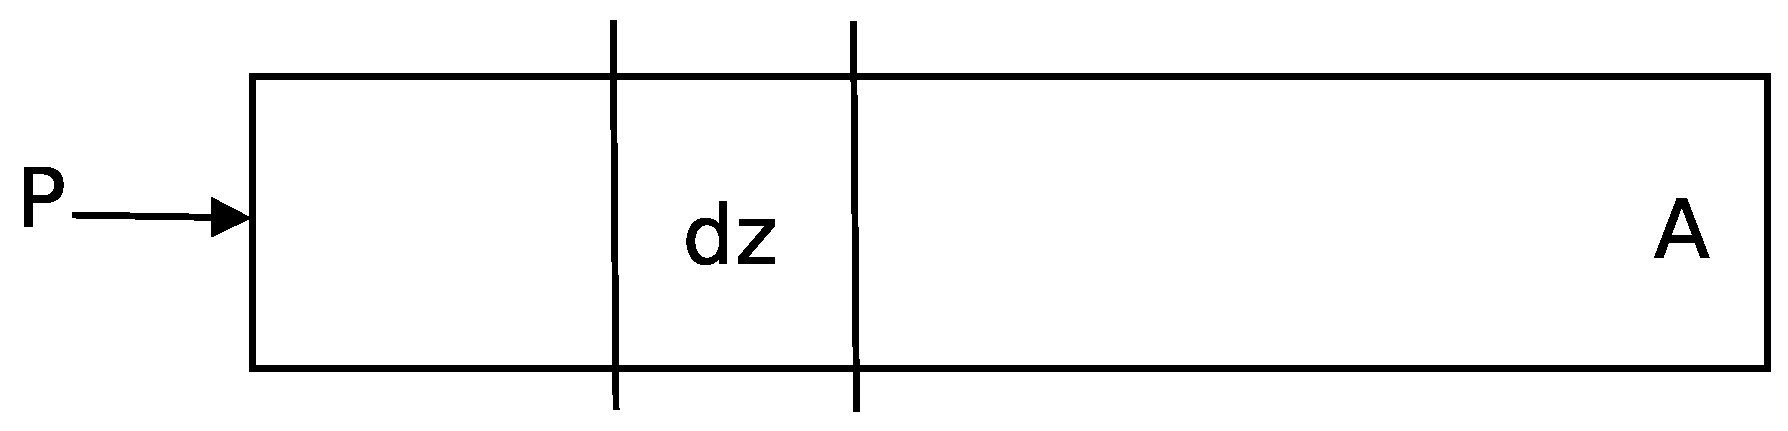
\includegraphics[width=0.8\textwidth]{eps_pics/deriveWaveRod}
\caption{Diagram for deriving the one dimensional wave equation given an axial pressure applied to one end of the material with uniform density and cross-sectional area.
	 \label{fig:deriveWaveRod}} 
\end{figure}

Figure \ref{fig:deriveWaveRod} gives a basic diagram that is used for the wave equation derivation, with $P$ being the axial pressure, $dz$ being the material's differential element of length, and $A$ being the cross-sectional area of the material. Define the stress in the z direction as:

\begin{equation}
T_3 = \frac{P}{A}
\end{equation}

\nomenclature{$P$}{Axial pressure applied to rod end}
\nomenclature{$A$}{Cross-sectional area of the rod}
\nomenclature{$dz$}{Differential element of length for the rod}
\nomenclature{$T_3$}{Stress in the z direction}

\begin{figure}[ht!]
\centering
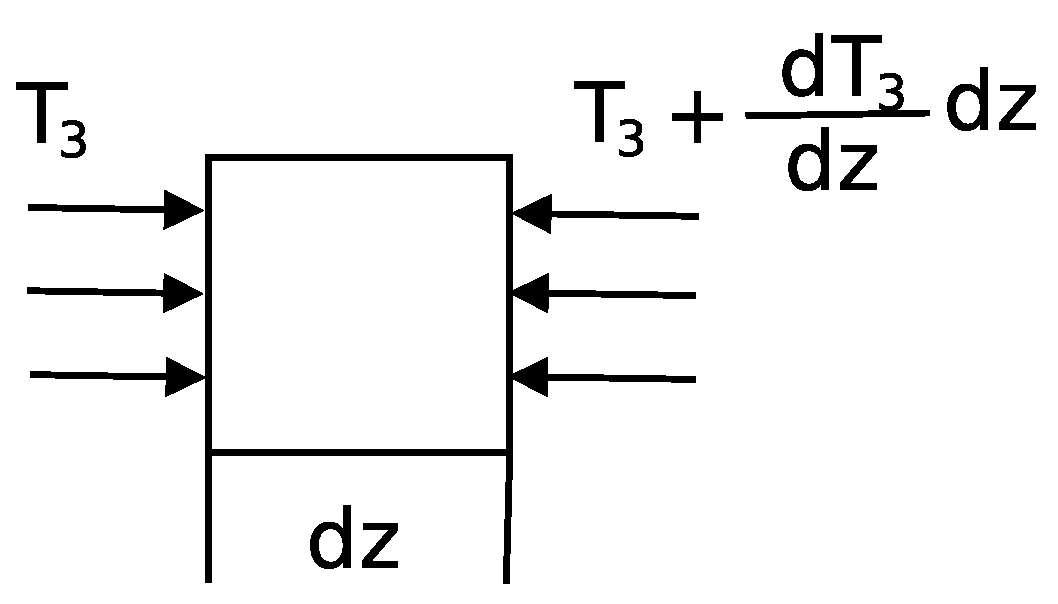
\includegraphics[width=0.8\textwidth]{eps_pics/diffElementRod}
\caption{Differential element showing the stresses acting on the rod.
	 \label{fig:diffElementRod}} 
\end{figure}

Applying Newton's second law and summing the forces,

\begin{equation}
-T_3A + (T_3 + \frac{dT_3}{dz}dz)A = A\rho dz \frac{d^2w}{dt^2}
\end{equation}

\nomenclature{$\rho$}{Density of the rod material}
\nomenclature{$w$}{Displacement of the rod}

With $\rho$ being the density of the rod material and $w$ being the displacement. Dividing through by the area,

\begin{equation}
-T_3 + T_3 + \frac{dT_3}{dz}dz = \rho dz \frac{d^2w}{dt^2}
\end{equation}

\begin{equation}
\frac{dT_3}{dz}dz = \rho dz \frac{d^2w}{dt^2}
\end{equation}

Canceling the $dz$ term,

\begin{equation}
\frac{dT_3}{dz} = \rho \frac{d^2w}{dt^2}
\label{eq:strainWave}
\end{equation}

$C_{33}$ is the elastic constant in the z direction and is defined as the ratio of the stress and strain in the z direction. This is given by,

\begin{equation}
C_{33} = \frac{T_3}{\epsilon_{33}} \implies T_3 = C_{33}\epsilon_{33}
\label{eq:T_3}
\end{equation}

\nomenclature{$C_{33}$}{Elastic constant in the z direction}
\nomenclature{$\epsilon_{33}$}{Strain in the z direction}

With $\epsilon_{33}$ being the strain in the z direction. Strain is the ratio of the change in material length to the original length and in this case is given by,

\begin{equation}
\epsilon_{33} = \frac{dw}{dz}
\label{eq:eps33}
\end{equation}

Inserting \ref{eq:eps33} in to \ref{eq:T_3} we see that

\begin{equation}
T_3 = C_{33}\frac{dw}{dz}
\label{eq:T_3fin}
\end{equation}

Putting \ref{eq:T_3fin} back in to \ref{eq:strainWave},

\begin{equation}
C_{33}\frac{d^2w}{dz^2} = \rho \frac{d^2w}{dt^2}
\end{equation}

Dividing through by $\rho$ and moving the LHS term to the RHS, we arrive at

\begin{equation}
\frac{d^2w}{dt^2} - c^2 \frac{d^2w}{dz^2} = 0
\label{eq:waveEquationFin}
\end{equation}

\nomenclature{$c$}{Velocity of wave propagation through the rod}

With $c$ being the velocity of the wave propagation and is defined as,

\begin{equation}
c = \sqrt{\frac{C_{33}}{\rho}}
\end{equation}

\section{Piezoelectric transducers with rod}

This section describes the governing equations for $d_{33}$ piezoelectric transducers that are placed on each end of a rod. The following work is based on derivations by Dr. Korde.

